\documentclass{beamer}

\usepackage{xcolor}
\usepackage{graphicx}
\usepackage{varwidth}
% \usepackage{caption}

\usepackage{subcaption}
\usepackage{media9}
\usepackage{multimedia}

\usepackage{amsfonts,amsmath,amssymb}
\usepackage{blkarray,booktabs,bigstrut}

\usepackage{pgfplots}
\usepackage{tikz}
\usepackage{filecontents}
\usepackage{lmodern}

% A latex package for displaying Julia code using the listings package.
% https://github.com/wg030/jlcode
% \usepackage{jlcode}

\usetikzlibrary{hobby}
\usetikzlibrary{decorations.shapes}
\usetikzlibrary{shadows.blur}

\definecolor{NvidiaGreen}{RGB}{118, 185, 0}

\usetheme{Madrid}
\setbeamertemplate{navigation symbols}{}

% Set the colors for various Beamer elements
\setbeamercolor{title}{fg=black, bg=NvidiaGreen} 
\setbeamercolor{frametitle}{fg=black, bg=NvidiaGreen} 
\setbeamercolor{item}{fg=black, bg=NvidiaGreen} 
\setbeamercolor{section in toc}{fg=black, bg=NvidiaGreen}
\setbeamercolor{author}{fg=white, 
        % bg=NvidiaGreen
    }
\setbeamercolor{date}{fg=white, 
        % bg=NvidiaGreen
    }

% Set the background to white for a clean presentation
\setbeamercolor{background canvas}{bg=white}

% #########################################################################################
% #########################################################################################
% Title
% #########################################################################################
% #########################################################################################

\begin{document}
{
\setbeamertemplate{background} 
{
    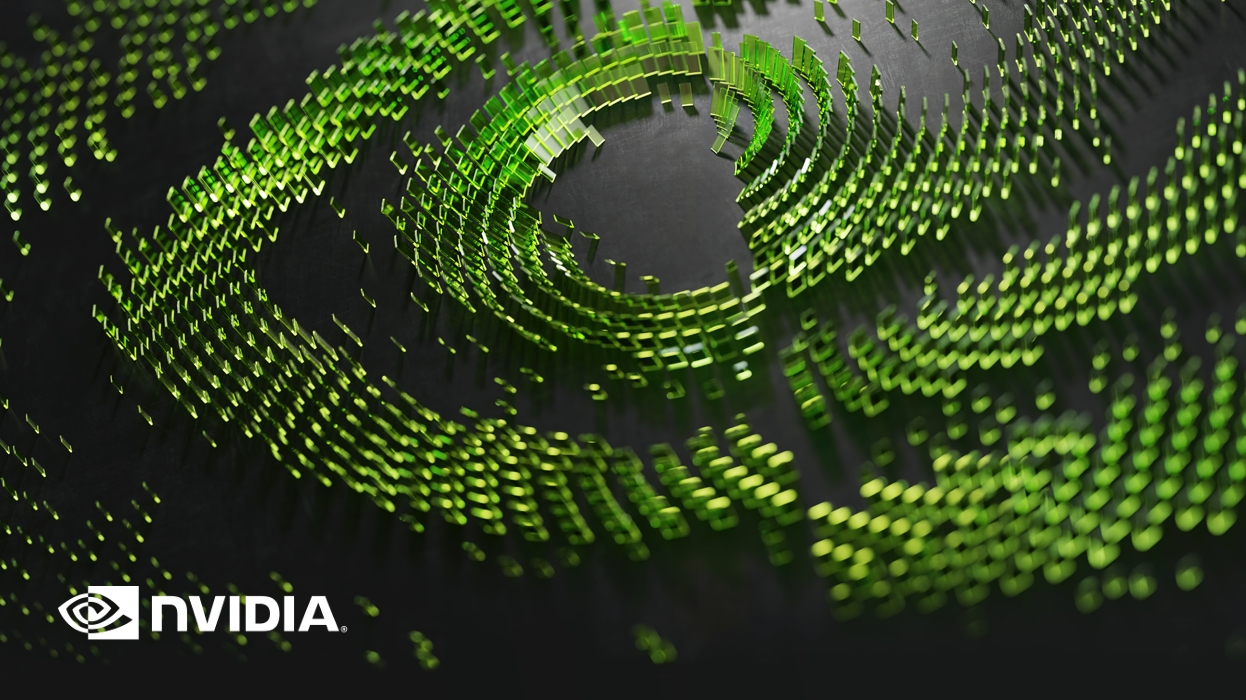
\includegraphics[width=\paperwidth,height=\paperheight]{images/Screenshot_9-12-2024_212019_.jpeg}
}
\title{\textbf{Lecture 15 - Spectral Clustering}}
\author[]{\textbf{Renan Monteiro Barbosa}}
% \date{\today}
\date[]{\textbf{2025}}
\maketitle
}

% #########################################################################################
% #########################################################################################
% Slide 1 - Intro
% #########################################################################################
% #########################################################################################

\section{Spectral Clustering}
\begin{frame}
\frametitle{\textbf{Spectral Clustering} }

Let G be a graph, $G(V,E)$, where $V = \left\{1,2,3, \cdots, n\right\}$ \vspace{0.2 cm}

The Laplacian matrix: 
% \parbox{4em}
\[
L_{G} = \underbrace{D_{G}}_{\parbox{3cm}{\centering Diagonal matrix \\[-3pt] with degrees of each vertex}} - \underbrace{A_{G}}_{\text{adjancency matrix}}
\]

$L_{G}$ is a PSD Matrix whose eigenvalues are

\begin{equation*}
    0 = \lambda_1 \leq \underbrace{\lambda_2}_{\text{Fiedler value}}\leq \lambda_3 \leq \cdots \leq \lambda_n
\end{equation*}

An eigenvector with eigenvalue $\lambda_2$ is called the \underline{Fiedler vector} of $\vec{W}$.


\end{frame}

% #########################################################################################
% #########################################################################################
% Slide 2 - Intro
% #########################################################################################
% #########################################################################################

\section{Spectral Clustering}
\begin{frame}
\frametitle{\textbf{Spectral Clustering} }

We will use $\vec{W}$, $L_{G}$ to understand clusters in a graph. \vspace{0.5 cm}

% Need to draw the graph clusters and draw the circle

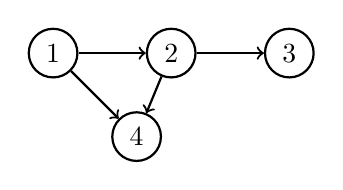
\begin{tikzpicture}[node distance={15mm}, thick, main/.style = {draw, circle}] 
    \node[main] (1) {$1$}; 
    \node[main] (2) [right of=1] {$2$}; 
    \node[main] (3) [right of=2] {$3$}; 
    \node[main] (4) [below right of=1] {$4$}; 
    \draw[->] (1) -- (2); 
    \draw[->] (1) -- (4);  
    \draw[->] (2) -- (3); 
    \draw[->] (2) -- (4); 
\end{tikzpicture}

$A = \left\{4,5,6,7,8\right\} , |A| = 5$

Notation

If X, Y are sets $X \ Y = \left\{x \in X | x \notin Y\right\}$

$|x| = \text{size of x}$



\end{frame}

% #########################################################################################
% #########################################################################################
% Slide 3 - Cut
% #########################################################################################
% #########################################################################################

\section{Cut}
\begin{frame}
\frametitle{\textbf{Cut} }
\textbf{Definition} \vspace{0.2 cm}

A cut is G is a partition of V into two sets, A and V \ A, when $A V$. (The cut induced by A)

\textbf{Notation} \vspace{0.2 cm}

If $X,Y V$, let E(X,Y) denote all edges with one certex in X and one vertex in Y.

$E(A, V \ A) = \left\{ \left\{1,6\right\} \right\}$


Definition

The density of the cut induced by A is:



\end{frame}

% #########################################################################################
% #########################################################################################
% Slide 4 - Sparsest cut
% #########################################################################################
% #########################################################################################

\section{Sparsest cut}
\begin{frame}
\frametitle{\textbf{Sparsest cut} }
Definition: \vspace{0.2 cm}

Let denote the smallest possible desnity of ca cut in G. Any cut with density is called a sparesest cut in G.

\end{frame}

% #########################################################################################
% #########################################################################################
% Slide 5 - Example in Julia
% #########################################################################################
% #########################################################################################

\section{Example in Julia}
\begin{frame}
\frametitle{\textbf{Example in Julia} }

Need to figure out how to make code look pretty in Latex

\end{frame}

% #########################################################################################
% #########################################################################################
% Slide 6 - Exploring
% #########################################################################################
% #########################################################################################

\section{Exploring}
\begin{frame}
\frametitle{\textbf{Exploring} }

\begin{equation*}
    Q\left(\vec{x}\right) = n \cdot \frac{ \sum_{\left\{i,j\right\} \in E\left(G\right) } \left(x_{i}-x_{j}\right)^2}{ \sum_{1 \leq i < j \leq n} \left(x_{i}-x_{j}\right)^2}
\end{equation*}

Let $A \subseteq V$, 

$A = \left\{4,5,6,7,8\right\}$, $\vec{C}_A = 
\begin{pmatrix} 
    0 \\ 
    0 \\ 
    0 \\ 
    1 \\
    1 \\
    1 \\
    1 \\
    0 \\
    0
\end{pmatrix}
$

\end{frame}

% #########################################################################################
% #########################################################################################
% Slide 6 - Exploring
% #########################################################################################
% #########################################################################################

\section{Exploring}
\begin{frame}
\frametitle{\textbf{Exploring} }

Need to add a visual representation demonstrating the Graph Laplacian and the example in code. About the information we can extract from the Graph Laplacian.

\end{frame}

% #########################################################################################
% #########################################################################################
% Slide XX - Conclusion
% #########################################################################################
% #########################################################################################

\section{Conclusion}
\begin{frame}
\frametitle{Conclusion}

here we go: \vspace{0.2 cm}

% % displayed code
% \begin{jllisting}
%     # some julia code
%     println( "Here we go with Julia!")
% \end{jllisting}

\end{frame}


% #########################################################################################
% #########################################################################################
% #########################################################################################
% #########################################################################################

% ⠀⠀⠀⠀⠀⠀⠀⠀⠀⠀⠀⠀⠀⣀⣀⣀⡀⠀⠀⠀⠀⠀⠀⠀⠀⠀
% ⠀⠀⠀⠀⠀⠀⢀⣠⠤⠖⠈⠉⠉⠀⠀⠀⠀⠉⠢⡀⠀⠀⠀⠀⠀⠀
% ⠀⠀⠀⠀⠀⣴⠏⠀⠀⠀⠀⠀⠀⠀⠀⠀⠀⠀⠀⠈⢦⡀⠀⠀⠀⠀
% ⠀⠀⠀⣠⠞⠁⠀⠀⠀⠀⠀⠀⠀⠀⠀⢀⠞⠋⢙⣦⡈⣷⡄⠀⠀⠀
% ⠀⣀⠶⠁⠀⠀⣀⣀⡀⠀⠀⠀⠀⠀⡴⠁⠀⠀⠿⢿⡟⣌⢿⠀⠀⠀
% ⣠⡿⠀⢠⣜⠉⠀⠀⠙⢷⢄⠀⠀⠀⢧⠀⠀⠀⠀⠀⠀⠘⡆⢧⡀⠀
% ⣯⠃⠀⢾⣿⠗⠀⠀⠀⠀⡽⠀⠀⠀⠈⠳⢄⣀⠀⠀⠀⡰⠃⠘⣵⡄
% ⡏⠀⠀⠘⡄⠀⠀⠀⣠⠞⠁⠀⠀⠀⠀⠀⠀⠀⠉⠉⠁⠀⠀⠀⢱⡇
% ⡅⠀⠀⠀⠙⠒⠔⠚⠁⠀⠀⠀⠀⠀⠀⠀⠀⠀⠀⠀⠀⠀⠀⠀⠀⡇
% ⣧⡀⠀⠀⠀⠀⠀⠀⠀⠀⠀⠀⠀⠀⠀⠀⠀⢠⠀⠀⠀⠀⠀⠀⠀⡗
% ⡿⡇⠀⠀⠀⠀⠀⠀⠀⠀⠀⢠⡀⠀⠀⠀⠀⢸⡇⠀⠀⠀⠀⠀⠀⣇
% ⠹⣷⠀⠀⠀⠀⠀⠀⠀⠀⠀⠈⠷⣤⣤⣤⣤⠞⠁⠀⠀⠀⠀⠀⠀⣸
% ⠀⠸⣇⠀⠀⠀⠀⠀⠀⠀⠀⠀⠀⠀⠀⠀⠀⠀⠀⠀⠀⠀⠀⠀⣰⠇
% ⠀⠀⢇⠳⣄⠀⠀⠀⠀⠀⠀⠀⠀⠀⠀⠀⠀⠀⠀⠀⠀⠀⠀⢀⡏⠀
% ⠀⠀⠈⠀⠀⠉⠀⠀⠀⠀⠀⠀⠀⠀⠀⠀⠀⠀⠀⠀

% #########################################################################################
% #########################################################################################
% #########################################################################################
% #########################################################################################

\end{document}